\section{Reading Comprehension}

\subsection{Definition}
A machine comprehends a passage of text if, for any question regarding that text that can be answered correctly by a majority of native speakers, that machine can provide a string which those speakers would agree both answers that question, and does not contain information irrelevant to that question.

\subsection{Recent Work}
The recent work in augmented RNN architectures in \ref{section:augmented} have achieved a great progress in question answering and reading comprehension tasks.

\subsection{Attentive Reader}
One architecture\cite{DBLP:journals/corr/ChenBM16a} for machine comprehension which summarises both the question and passage(context) into high level representation of vectors using RNN cells and then tries to predict the best span of text that contains the answer. 

\begin{figure}[H]%
      \center%
        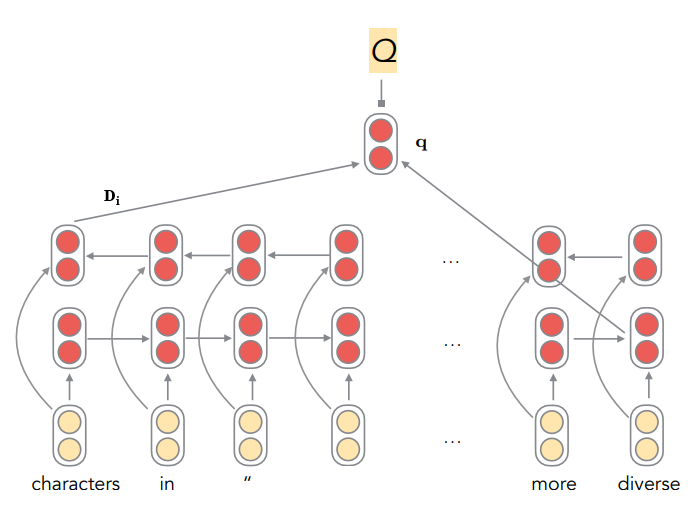
\includegraphics[width=.7\textwidth]{images/komy/attentive-reader.png}%
        % you need to add the caption for the list of figures
        \caption[Attentive Reader]{An Attentive Reader}%\label{fig:a}%
  \end{figure}